\section{Micro-P4 \;($\mu$P4)}
Re-configurable targets process packets using multiple type of processing blocks and P4 provides multiple sub-languages following heterogenous abstract machines to program the blocks.
The presence of heterogeneous abstract-machines and device-specific constructs is the
primary reason for lack of mechanisms for modularity and code reuse.
Because, it is not possible to define interface to reuse code modules when caller and callee modules can have incompatible abstract machines.


$\mu$P4 comprise of an architecture, $\mu$SA, and a compiler, $\mu$P4C for a logical target device. 
$\mu$SA simplifies abstract machine for P4 data plane programs by exposing minimal number of programmable blocks required to implement.
It provides abstraction by defining logical externs that allows programmers to express packet-processing logic that is outside the scope of current P4 and relies on fixed-function blocks in real targets.
In $\mu$SA, we define generic interfaces to enable easy code reuse of fine-grained packet-processing functions and build new functions.
We associate runtime behavior with the generic interface as described in Section \ref{subsection:packet-processing-using-mp4}. 
$\mu$P4C allows programmer to express \emph{sequential} and \emph{parallel} execution multiple fine-grained functions.
Unlike Hyper4 and P4Visor, $\mu$P4C enables composition of packet-processing functions using P4 language itself without relying on different configuration languages.
It translates simplified abstract machine and its logical externs into real target-specific heterogeneous packet-processing blocks, features and constraints.


\subsection{Packet Processing using $\mu$P4}
\label{subsection:packet-processing-using-mp4}
We model every packet-processing function as a black-box micro-switch that processes packet byte-stream, intrinsic metadata and user-defined parameters as shown in Figure \ref{fig:package-runtime-behavior}.
The black-box model hides implementation details (headers types, user-defined metadata, programmable blocks etc.,) of micro-switch programs.
To realise this model, $\mu$SA defines multiple packet-processing pipelines and each pipeline is associated with one or more generic interface types.
Each generic interface exposes a set of programmable blocks to implement and allows programmers to specify type parameters for runtime arguments.
Programmers can implement the interfaces and define new \emph{package} types.
In control blocks of $\mu$SA pipelines, the package types can be instantiated and invoked by supplying arguments for the defined runtime parameters. 
\begin{figure}[!h]
    \centering
    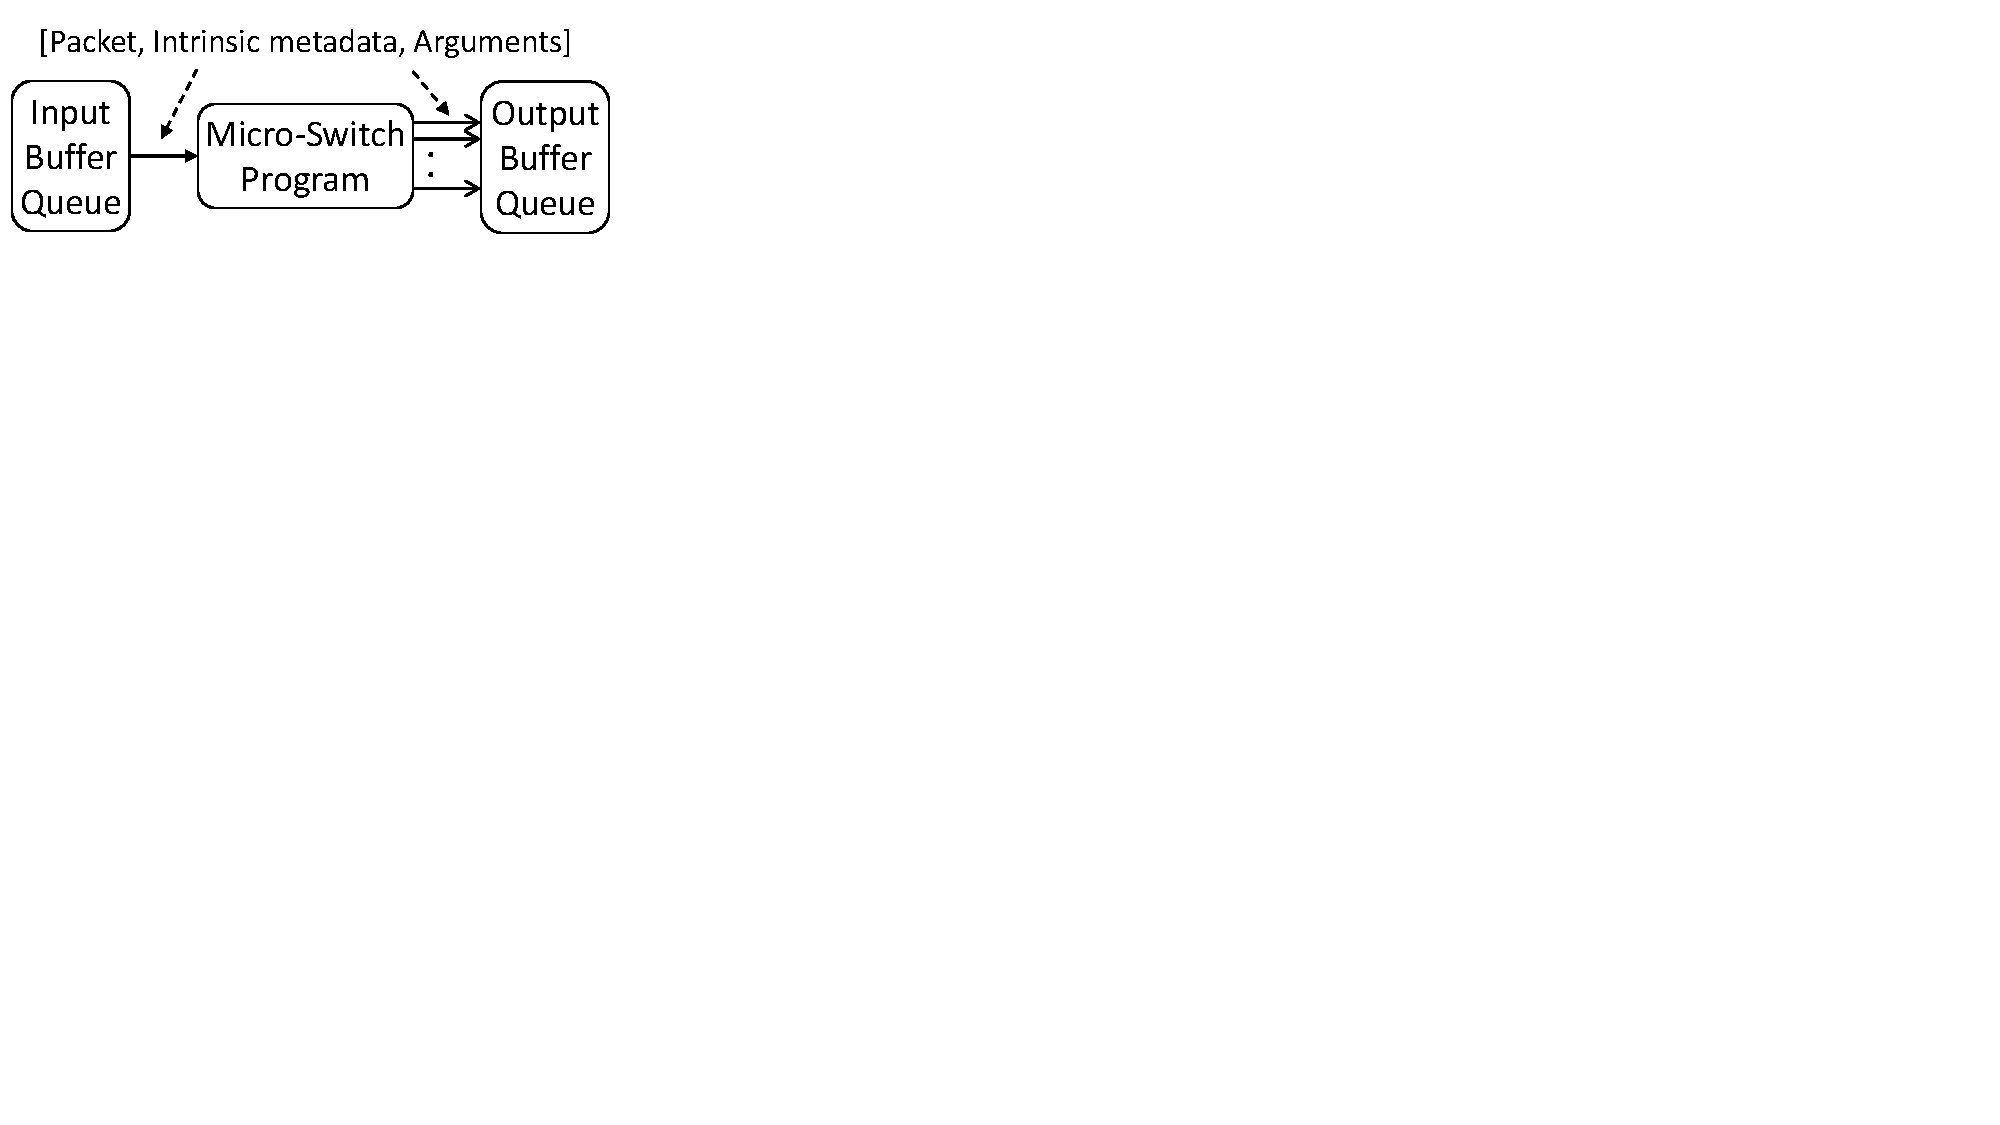
\includegraphics[trim=0 420 667 0, clip, scale=0.5]{microp4-program-model}
    \label{fig:package-runtime-behavior}
    \caption{Micro P4 Package Runtime Behavior}
\end{figure}

\begin{figure}[!h]
\begin{lstlisting}[frame=none]
// Signature of Runtime Interfaces
U<I, O, IO>(pkt_in, pkt_out, inout sm_t, es_t, in I, out O, inout IO); 
M<O>(pkt_in, in sm_t, es_t, out_buf<O>); 
G<I, O>(in_buf<I>, out_buf<O>); 
\end{lstlisting}
\caption{Runtime Interfaces}
\label{fig:interfaces}
\end{figure}

\subsubsection{Sequential Execution}
\label{subsubsection:sequential-execution}
Sequential execution of micro-switch programs follow a single-thread model.
Only one micro-switch program processes a packet at a time.
$\mu$P4 allows programmers to invoke micro-switch programs using their interfaces in body of control blocks other micro-switch program.
Programmers can logical externs defined in $\mu$SA to express sequential processing.
Figure \ref{fig:sequential-execution} illustrates reuse of the code shown in Figure \ref{fig:l3.p4.l2.p4} to build a routing function, called emph{l2l3}.
 \begin{figure}[ht]
\begin{lstlisting}[frame=none]
// interfaces for l3 and l2
l3(pkt_in, pkt_out, sm_t, es_t, out bit<16>);
l2(pkt_in, pkt_out, sm_t, es_t, in bit<16>);

control l2l3(pkt_in pin, pkt_out po, 
             sm_t s, es_t e) {
  bit<16> next_hop; pkt_in pin_l2;
  apply {
    l3.apply(pi, po, s, es, next_hop);
    // sets `pin_l2' with `po's bytes, resets `po'
    po.get_pkt_in(pin_l2); // extern method call
    l2.apply(pin_l2, po, s, es, next_hop);
  }
}
\end{lstlisting}
\caption{Sequential Execution}
\label{fig:sequential-execution}
\end{figure}

\subsubsection{Parallel Execution}
\label{subsubsection:parallel-execution}
In parallel execution of multiple micro-switch programs, each program processes its own copy of a packet.
Programmers can create copies of a packet using logical constructs defined in $\mu$SA.
Figure \ref{fig:parallel-execution} shows a code snippet of a micro-switch program, called \emph{rm}, performing routing and mirroring.
It executes micro-programs \emph{l2l3} (Figure \ref{fig:sequential-execution}) and \emph{mirror} (samples traffic) in parallel.
\begin{figure}[ht]
\begin{lstlisting}[frame=none]
// interface for traffic mirror function
mirror (pkt_in, pkt_out, sm_t);
l2l3 (pkt_in, pkt_out, sm_t);
struct e_t {};
control rm(in_buf<e_t> ib, out_buf<e_t> ob) {
  pkt_in pin, pin_m; es_t es_m;
  pkt_out po_m; sm_t sm, sm_m;
  apply {
    ib.dequeue(pin, sm, es);
    // copies for parallel execution
    pin_m.copy_from(pin); sm_m = sm; 
    es_m.copy_from(es)
    mirror.apply(pin_m, po_m, sm_m, es_m);
    l2l3.apply(pin, po, sm, es);
    // synchronize and put in out_buf arg
    ob.enqueue(po, sm, es);
    ob.enqueue(po_m, sm_m, es_m);
  }
}
\end{lstlisting}
\caption{Parallel Execution}
\label{fig:parallel-execution}
\end{figure}

\subsubsection{Multicast Execution}
\label{subsubsection:multicast-execution}
Multicast execution differs from parallel execution in two fundamental aspects.
$(1)$ Multicast execution allows to program packet replication at runtime.
$(2)$ Each copy of the replicated packet executes the same code.
% $\mu$SA defines a logical multicast engine, \texttt{mc\_engine\_t}, as an extern.
Figure \ref{fig:multicast-execution} shows an example of expressing multicast replication using logical externs defined in $\mu$SA.
\begin{figure}[ht]
\begin{lstlisting}[frame=none]
struct out_t { bit<16> data;}
control mc(pkt_in pi, sm_t sm, es_t es, 
        hs_t h, ia_t ia, mc_buf<hs_t, out_t> hb) {
  mc_engine_t mce;  pkt_inst_id_t id; 
  out_t  oa;
  table t{
    key = {} actions = { mce.set_mc_group; drop; }
  }
  table mac{
    key = { es.get_port(); } 
    actions = { mac_update; }
  }
  apply {
    id = mce.apply(es); // equivalent to fork in C
    mac.apply();
    hb.enqueue(h, sm, es, oa);
  }
}
control dep(pkt_out<o_a> ob, 
            mc_buf<hs_t, out_arg_t> hb) {
  hs_t hdrs; out_arg_t oa; pkt_out po;
  hb.dequeue(hdrs, sm, es, oa);
  // deparser code 
  ob.enqueue(po, sm, es, oa);
}
\end{lstlisting}
\caption{Multicast Execution}
\label{fig:multicast-execution}
\end{figure}

\subsection{Compiling $\mu$P4 Programs}

\begin{figure}[!h]
    \begin{subfigure}{\linewidth}
        \centering
        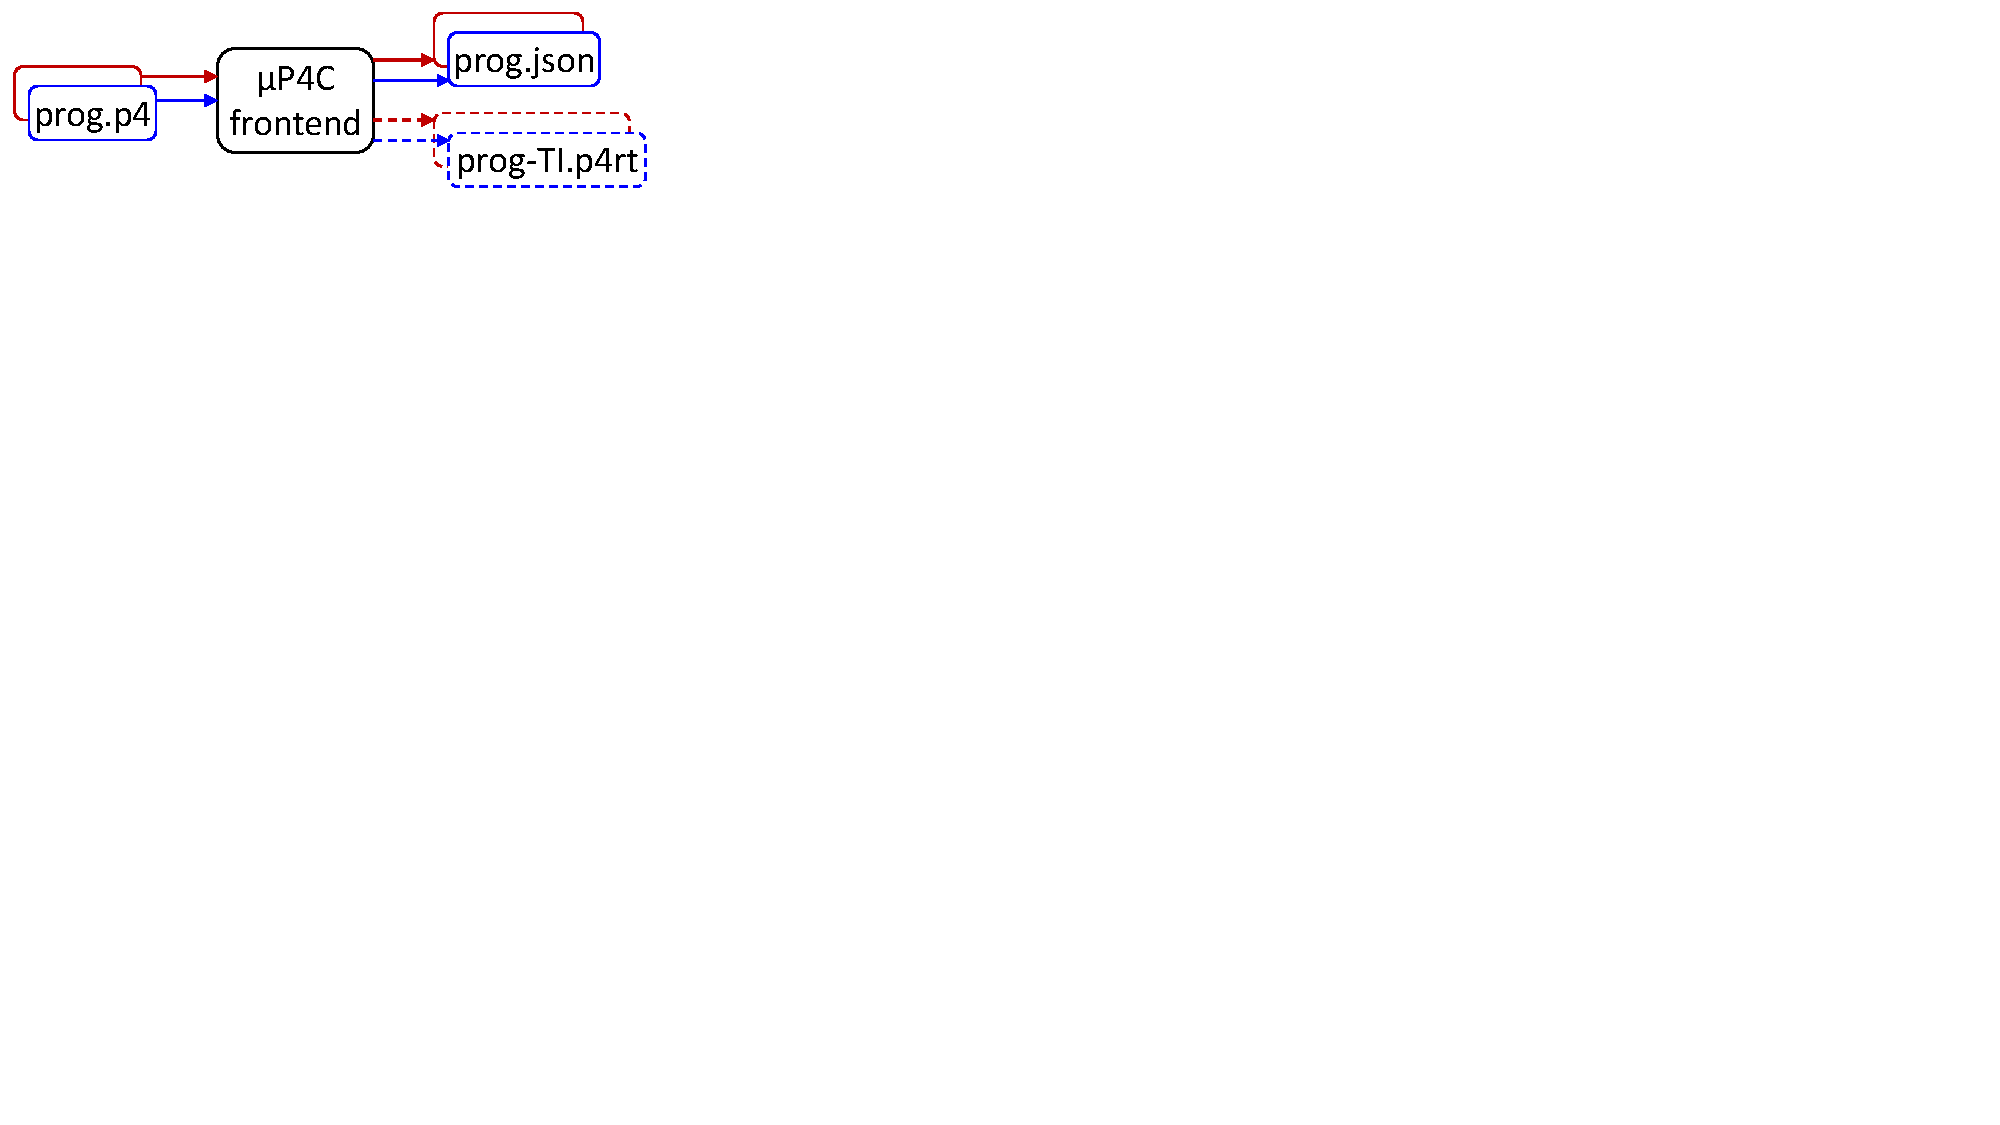
\includegraphics[trim=0 435 665 0, clip,scale=0.55]{mp4c-frontend}
        \caption{Library Program Compilation}
        \label{subfig:compiling-modules}
    \end{subfigure}
    \begin{subfigure}{\linewidth}
        \centering
        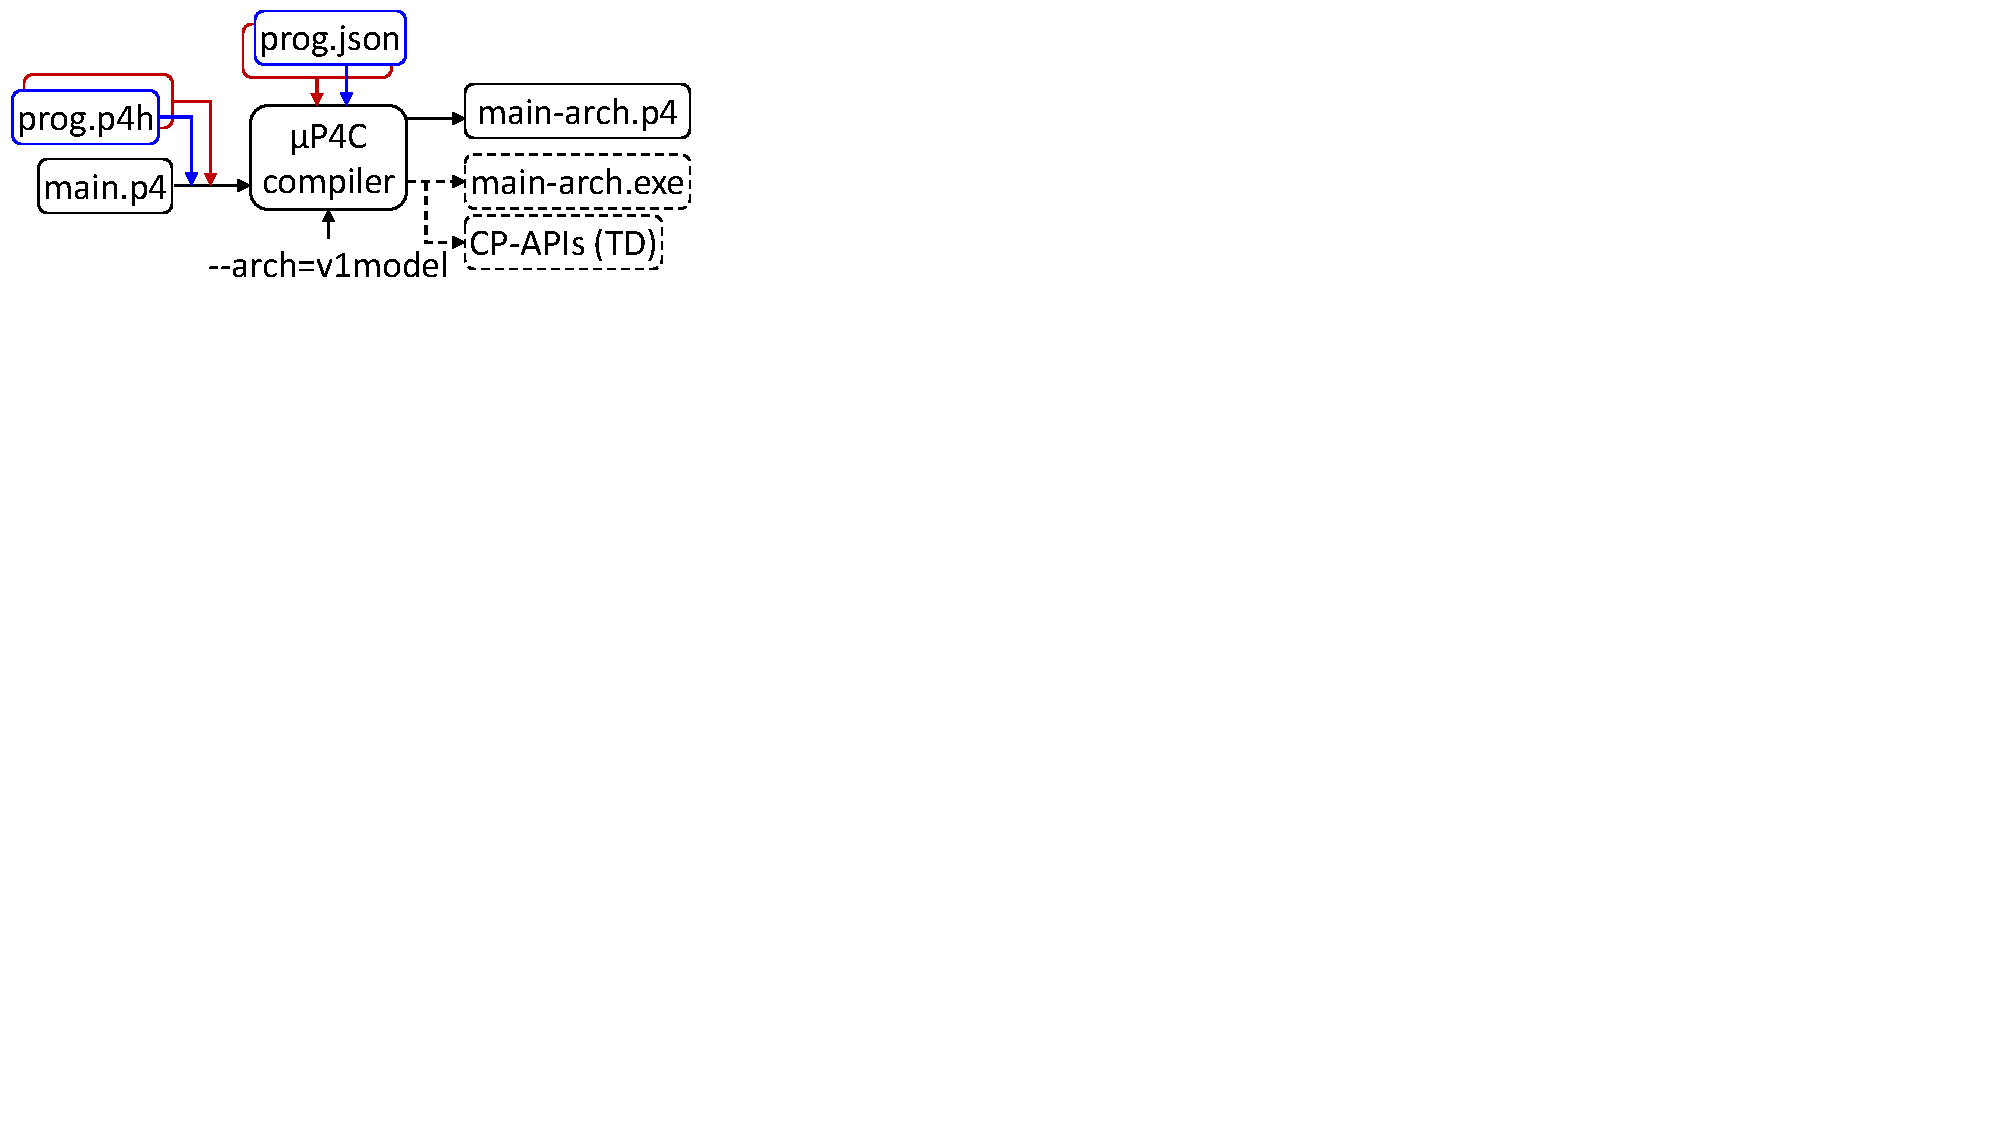
\includegraphics[trim=0 407 628 0, clip,scale=0.55]{mp4c-compiler}
        \caption{Composition and Translation of Main Instance}
        \label{subfig:composition-translation-of-main-instance}
    \end{subfigure}
\caption{Compiling $\mu$SA programs}
\label{fig:compiling-msa-programs}
\end{figure}
